\section{Overview}
\label{sec:overview}

\begin{figure}[!htb]
\centering
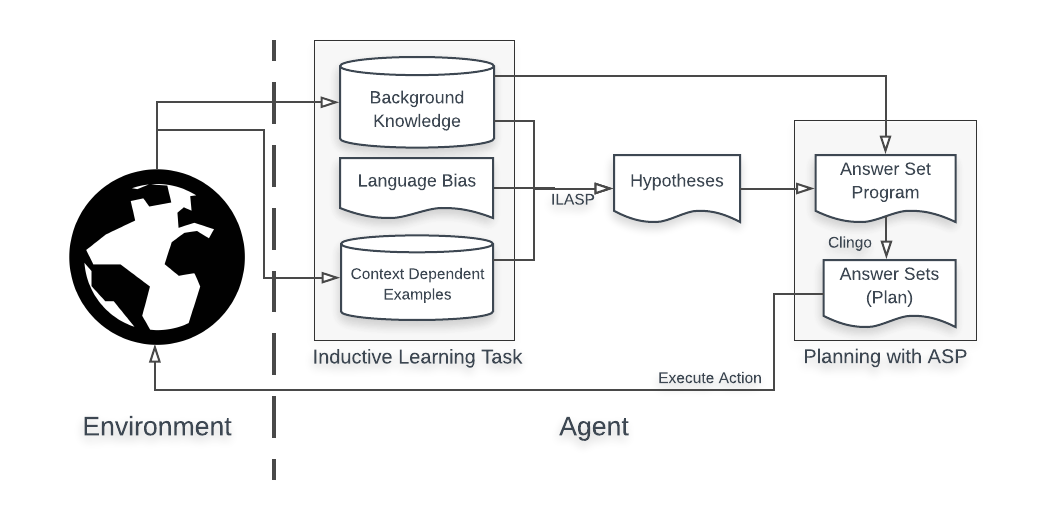
\includegraphics[width=1.0\textwidth]{./figures/architecture}
\caption{ILP(RL) overview}
\label{fig:ILPRL_overview}
\end{figure}

The overall architecture of the learning framework, called \textit{ILP(RL)}, is shown in Figure \ref{fig:ILPRL_overview}. 
By interacting with the environment, an agent receives state transition experiences as positive examples, which is used by ILASP, together with pre-defined background knowledge and language bias, to learn and improve hypotheses.
The agent also remembers surrounding information it has seen as background knowledge, which is used to make an action plan together using the learnt hypotheses by solving an answer set program.
Mechanisms of each step is explained in details in the following sections.

\section{Inductive Learning Tasks}
\label{sec:inductive_learning_tasks}

% \textcolor{red}{Draw an illustration of the difference between exploration and las part}\\
% \textcolor{red}{Related these with Definition of ILASP}\\

The first step is to translate experiences generated by the interaction with an environment into ASP syntax. 
Similar to an existing RL, an agent explores an environment following an exploration strategy.
Every time the agent takes an action, these experiences are recorded in two different forms: 
a positive example and background knowledge. 
Positive examples and background knowledge are used by ILASP for inductive learning, and background knowledge is used by both ILASP and ASP for solving for answer sets.
Thus it is necessary to convert them into ASP syntax.

The full details for ILASP learning tasks is described in Appendix XXX.

\subsection{Context Dependent Examples}
Context dependent examples contain information about how the state transitions between the current state and the next state.
They are equivalent to context-dependent partial interpretation (CDPI) in  $ILP_{LAS}^{context}$. 
As defined in the Equation \ref{eq:cdpi}, CDPI is of the form $\langle$ e, C $\rangle$ where e = $\langle$ e\textsuperscript{inc}, e\textsuperscript{exc} $\rangle$. 
Each of the components in CDPI is defined as follows:
\begin{defn}
e\textsuperscript{inc} of CDPI for ILP(RL) is the next state of an agent $\forall$ s\textsubscript{t+1} $\in$ S such that answer sets of B $\cup$ H does not cover.
\end{defn}

\begin{defn} \label{def:ILPRL_context}
e\textsuperscript{exc} of CDPI for ILP(RL) is the next state of an agent $\forall$ s\textsubscript{t+1} $\not\in$ S such that answer sets of B $\cup$ H covers,
as well as $\forall$ s$^\prime$\textsubscript{t+1} $\in$ S\textsubscript{neighbor} such that s\textsubscript{t+1} $\neq$ s$^\prime$\textsubscript{t+1}.
\end{defn}
where B is the current background knowledge, H is the current hypotheses learnt by previous inductive learning using ILASP, S is all the states in the environment, and S\textsubscript{neighbor} is all adjacent states of s\textsubscript{t} as well as s\textsubscript{t} itself.

\begin{defn}
Context C of CDPI for ILP(RL) contains an action a\textsubscript{t}, a state s\textsubscript{t}, and adjacent walls of s\textsubscript{t}.
\label{def:context}
\end{defn}

In this paper, we assume that part of context contains only whether a wall exists or not, with the presence of a wall, the agent cannot move to the state where a wall exist.

\subsubsection{Positive examples in ASP syntax}
\label{subsubsec:positive_examples_asp_syntax}
A positive example is expressed as a following ASP form:
\begin{equation}
\begin{split}
    \textsf{\#pos}(\{e\textsuperscript{inc}\}, \{e\textsuperscript{exc}\}, \textsf{\{C\}})
\end{split}
\end{equation}

For e\textsuperscript{inc} and e\textsuperscript{exc}, s\textsubscript{t+1} is expressed as \textit{state\_after((x,y))}, where x and y represent coodinates of X and Y axis in an environment respectively.
Thus both e\textsuperscript{inc} and e\textsuperscript{exc} contain only state\_after((x,y)) or empty.
For context C, a\textsubscript{t} is translated int \textit{action((a))}, s\textsubscript{t} is translated into \textit{state\_before((x,y))}, and adjacent walls of s\textsubscript{t} are translated into \textit{wall((x$^\prime$,y$^\prime$))}.

% For example, if the agent takes an action "up" to move from (1,1) to (1,2), all other states that the agent could have taken but did not are exclusions ((1,0), (1,1), (0,1) and (2,1) in this case).
% context examples include state\_before((X1,Y1)), which represents the position of the agent in x and y axis before an action is taken,
% action(A) is the action the agent has taken, and surrounding information, such as surrounding walls.

% Rewards are not used.
% (Discussed in details in Chapter XX).

% \textcolor{red}{There is no negative example as XXXX.}
% Using these positive examples, the agent is able to learn and improve hypothesis as it explore the environment and encounters new scenarios.
\begin{examp} \normalfont (Positive examples).

\begin{figure}[!htb]
\centering
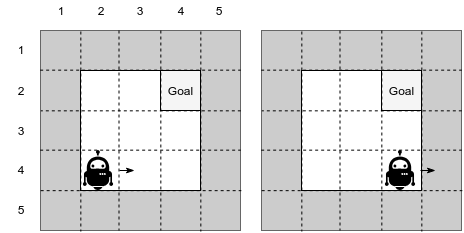
\includegraphics[width=0.7\textwidth]{./figures/pipeline_example1}
\caption{5$\times$5 grid world example}
\label{example_pos_example}
\end{figure}

We use a simple 5x5 gridworld environment to hilight how an agent gains a positive example, suppose the agent takes an action "right" to move from (2,4) to (3,4) cell, as shown on Figure \ref{example_pos_example} on the right.
All other alternative states that the agent could have ended up by taking different actions
(down, up, and left) are in the exclusions.
Context examples are the state that the agent is before taking an action and surrounding walls information. The following positive example is generated.

\begin{equation}
\begin{split}
    \textsf{\#pos(} & \textsf{\{state\_after((3,4))\},}\\
                    & \textsf{\{state\_after((2,4)),state\_after((1,5)),state\_after((0,4)),state\_after((1,4))\},} \\
    & \textsf{\{state\_before((2,4)). action(right). wall((1, 4)). wall((4, 2)).\})}
\end{split}
\end{equation}

This example will be used to learn how to move up as one of the agent's hypotheses.

Similarly, the agent is at (4,4) and tries to move right, as shown on the left on Figure \ref{example_pos_example}. In this case, however, there is a wall at (5,4) and therefore the agent ends up in the same state. From this example, the following positive example is generated:

\begin{equation}
\begin{split}
\textsf{\#pos(} & \textsf{\{state\_after((4,4))\}}, \\
                & \textsf{\{state\_after((4,3)),state\_after((3,4)),state\_after((5,4)),state\_after((4,5))\}} \\
                & \textsf{\{state\_before((4,4)). action(right). wall((5,4)). wall((4,5)).\}).}
\end{split}
\end{equation}

\end{examp}
\label{state_transition_example}

\subsection{Background Knowledge}
Having defined the positive examples, we now define necessary background knowledge for inductive learning.
In order to learn valid move for each direction in the form of state transition, it needs to know how it means to be "being next to XX".
The definition of \textsf{adjacent} is given as follows:

\begin{equation} \label{eq:adjacent}
\begin{split}
&\textsf{adjacent(right, (X+1,Y),(X,Y)) :- cell((X,Y)), cell((X+1,Y)).} \\
&\textsf{adjacent(left,(X,Y),  (X+1,Y)) :- cell((X,Y)), cell((X+1,Y)).} \\
&\textsf{adjacent(down, (X,Y+1),(X,Y)) :- cell((X,Y)), cell((X,Y+1)).} \\
&\textsf{adjacent(up,   (X,Y),  (X,Y+1)) :- cell((X,Y)), cell((X,Y+1)).} \\
\end{split}
\end{equation}

% Future research will relax these assumptions and attemp to learn more general hypothesis,
% e.g learning adjacent defintion.
In existing RL methods, the agent is only able to see the state where the agent is at, and this is an additional assumption that the agent is able to see surrounding states.
These adjacent concepts themselves could be learnt using ILASP separately, but in this preliminary research we focus on learning valid move, and this extension will be discussed in Further Research in XX.
In addition, \textit{cell((X,Y))} is defined as follows:
\begin{equation} \label{eq:cell}
\begin{split}
    &\textsf{cell((0..X, 0..Y)).}
\end{split}
\end{equation}

where, 0..X defines the range of X coodinates and X and Y are the size of width and height of the environment respectively. 
For 5x5 gridworld environment, for example, cell is defined as cell((0..5, 0..5)).

% While the agent explores the environment, it also keeps all the surrounding information as background knowledge,
% which will be stored in different repository, and are later used to generate a sequence of actions plan using H.

% This does not include state transition experience, as these state\_before and action takens are different at every timestep.
% In static environment (e.g no moving enermy), environment information remain the same across time, and thus it will be beneficial to remember.
% This principle is different from most RL methods, as they are model-free learning.
% As described in XX,, model-based learning converge to optimal policy more efficiently.

% In our simple maze environment, the agent is able to see the surrounding states and 
% these could be all wall position that the agent has seen so far, which can be
% wall((1, 5)). which represents the location of the wall.
% Another example could be a location of a teleportation if the agent sees it.
% These environment experiences are part of context examples in the positive examples.
\begin{examp} \normalfont (Background Knowledge).

XXX
% Using the same example as in Figure \ref{example_pos_example},
% The first postive examples contain two walls, wall((1,4)) and wall((4,2)), and they will be stored as background knoledge. These information are useful for the plan generation.
\end{examp}

\subsection{Language Bias}
\label{subsec:language_bias}
Recall in \ref{def:las_context} that H $\subseteq$ S\textsubscript{M} for $ILP_{LAS}^{context}$, thus we define a search space using a language bias specified by \textit{mode declaration}.
We define S\textsubscript{M} as follows:
\begin{equation} \label{eq:sm}
\begin{split}
&\textsf{\#modeh(state\_after(var(cell))).}\\
&\textsf{\#modeb(1, adjacent(const(action), var(cell), var(cell)), (positive)).} \\
&\textsf{\#modeb(1, state\_before(var(cell)), (positive)).} \\
&\textsf{\#modeb(1, action(const(action)),(positive)).} \\
&\textsf{\#modeb(1, wall(var(cell))).} \\
\end{split}
\end{equation}
% Without these in the form of mode bias, the search space for ILASP will be empty.

\textsf{\#modeh} and \textsf{\#modeb} are the \textit{normal head} declarations and the body declarations. 
The first argument of each \textsf{\#modeb} specifies the maximum number of times that \textsf{\#modeb} can be used in each rule (also called \textit{recall}), which is 1 in our case.  

\textsf{var(t)} is a placeholder for variable of \textit{type} \textsf{t}. In \ref{eq:sm}, we use \textsf{cell} for a variable type, which is based on any cell defined in \ref{eq:cell}.
\textsf{const(t)} is a placeholder for constant term of type \textsf{t}, and type \textsf{t} must be specified as \textsf{\#constant(t, c)}, where \textsf{c} is a constant term., 
const(t) is defined as follow:

\begin{equation}
\begin{split}
&\textsf{\#constant(action, right).}\\
&\textsf{\#constant(action, left).}\\
&\textsf{\#constant(action, down).}\\
&\textsf{\#constant(action, up).}
\end{split}
\end{equation}

\textsf{action} type is specified as constant since ILASP should learn different hypothesis for each action, and can be found in each context as specified in Definition \ref{def:context}.

\textsf{(positive)} in \textsf{\#modeb} specifies that the predicates only appears as positive and not negation as failure, which reduces the seach space. 
In this case, \textsf{\#modeb(1, wall(var(cell)))} could appears as \textsf{not wall}, and all other body declaration should be positive. 
% Positive excludes the possibility of negation as a failure in order to reduce the search space.

Finally, we define \textsf{\#max\_penalty} to specify the maximum size of the hypothesis. By default it is 15, and we increased to 50 as the maximum.
Increasing \#max\_penalty allows ILASP to learn longer hypothesis in expense of longer computation.
% As we describe in XXX, the search space increases in propotion to the complexity of learning tasks, which slows down the learning process.
% For example, the search space in this particular setting is in XX.
\begin{examp} \normalfont (Language Bias).

XXX
\end{examp}
    
\subsection{Hypothesis}
\label{sebsec:hypothesis}
Having defined the $ILP_{LAS}^{context}$ task T, ILP(RL) is able to learn an hypothesis H. 
Since B and S\textsubscript{M} are fixed, the learnt H varies depending on positive examples that the agent receives.
In the early phase of learning, the agent does not have many positive examples, and learns an hypothesis that is part of the full hypothesis that the agent can run in the environment.
Therefore it is important to iteratively improve hypotheses. Inductive learning algorithm is executed by the following rule.
\begin{defn}
ILP(RL) runs $ILP_{LAS}^{context}$ to relearn H\textsubscript{new} if and only if $\forall$$\langle$ e, C$\rangle$ $\in$ E\textsuperscript{+}, $\exists$A $\in$ Answer Sets (B $\cup$ C $\cup$ H) such that A extends e
\end{defn}
where H is the current hypothesis that the agent has learnt so far. 
Learnt hypotheses are improved when a new positive example is added and the current hypothesis does not cover the new positive example.
It it does cover it, there is no need to rerun ILASP again.

The learnt hypothesis will be used to generate a plan, which we describe in the next section.

\begin{examp} \normalfont (Hypothesis).

For example, if the agent has only one positive example,

XXX
This hypothesis, for example, does not explain how to move "down". In order to learn how to move "down", it needs an positive example of moving up.
\end{examp}

\section{Planning with Answer Set Programming}
\label{sec:planning}

Having learnt hypothesis using $ILP_{LAS}^{context}$, we can use the learnt hypotheses to generate a sequence of actions in the form of answer sets that the agent should follow.
In the following subsections, we explain how to create a answer set program and use the answer sets to make a plan in a maze.
\subsection{Constructin of Answer Set Program}
\label{subsec:construction_asp}
The ASP should be constructed such that answer sets of ASP are a sequence of actions and the next state by taking each action.

First, we use the learnt hypotheses by $ILP_{LAS}^{context}$ as rules for solving ASP.
In the  $ILP_{LAS}^{context}$, we only need to differenciate between s\textsubscript{t} and s\textsubscript{t+1} as \textsf{state\_before(T)} and \textsf{state\_after(T+1)} respectively.
However, for ASP planning, the answer sets contains a sequence of actions and states at each time steps. In order to capture the notion of time sequences, we modify the ASP syntax slightly by 
introducing T. Specifically, the following mapping is required 
\begin{equation}
\begin{split}
&\textsf{state\_after(V0) :- adjacent(right, V0, V1), state\_before(V1), action(right), not wall(V0).}\\
&\textsf{state\_after(V0) :- adjacent(left, V0, V1), state\_before(V1), action(left), not wall(V0).}\\
&\textsf{state\_after(V0) :- adjacent(down, V0, V1), state\_before(V1), action(down), not wall(V0).}\\
&\textsf{state\_after(V0) :- adjacent(up, V0, V1), state\_before(V1), action(up), not wall(V0).}
\end{split}
\end{equation}
% The syntax of ASP is different from ILASP phase, because we need to include time sequence when solving ASP.
% In ILASP, it is only state\_before and state\_after, but in plan generation, there will be more than one state transition.
% These syntax conversion needs to be done for learnt hypothesis    

\begin{examp} \normalfont (Mapping of ASP syntax between $ILP_{LAS}^{context}$ and ASP).

XXX
\end{examp}

Second, we define a rule for action, which is of the form:
\begin{equation}\label{eq:choice_rule}
\begin{split}
&\textsf{1\{action(down,T); action(up,T); action(right,T); action(left,T)\}1} \\
&\textsf{ :- time(T), not finished(T).}\\
\end{split}
\end{equation}

Action is given as a choice rule, and this choice rule states that action must be one of four actions: \textsf{down},\textsf{up},\textsf{right}, or \textsf{left}.
at each time step T, as defined maximum and minimum numbers in 1.
One of four actions must be selected unless \textsf{not finished(T)} or \textsf{time(T)} are satisfied, as defined in the body of the rule.
In RL scenarios, this means there is always action to be taken until the agent reaches a goal, thus \textsf{finished(T)} is satisfied, or time step T exceeds a maximum time step.
\begin{equation}
\begin{split}
&\textsf{time(T\textsubscript{t}..T\textsubscript{max})}
\end{split}
\end{equation}
where T\textsubscript{t} is the current time step and T\textsubscript{max} is the maximum time steps.
For example, if an agent is at time step 0, and can take actions 100 times to find a goal time is defined as \textsf{time(0..100)}.

\textsf{finished(T)} determines whether the agent reaches the goal, which is defined in the following ASP form:

\begin{equation}
\begin{split}
&\textsf{finished(T):- goal(T2), time(T), T} \geq \textsf{T2.}\\
&\textsf{goal(T):- state\_at((X\textsubscript{goal}, Y\textsubscript{goal}), T), not finished(T-1).}\\
&\textsf{goalMet:- goal(T).}\\
&\textsf{:- not goalMet.}
\end{split}
\end{equation}

\textsf{state\_at((X\textsubscript{goal}, Y\textsubscript{goal}))} is the location of the goal, which is unknown to the agent in the beginning of the training.
The agent explores the environment until it finds the goal location.
In the other word, the agent cannot generate a plan to the goal untile the goal is found. 
Once the agent reaches the goal and \textsf{finished(T)} is satisfied, 
there will not be any actions at time T+1 since the body of the action choice rule defined in \ref{eq:choice_rule} is not satisfied.

Next, facts of walls information is provided as follows:
\begin{equation}
\begin{split}
&\textsf{wall((X,Y))}\\
\end{split}
\end{equation}

As defined in Definition \ref{def:ILPRL_context}, the agent is assumed to be able to see ajacent walls and used it as a context in positive examples in $ILP_{LAS}^{context}$. 
For ASP planning part, these wall information is accumulated as background knowledge as a separate repository, and used it for solving ASP. 

Next, the starting state for the planning provided as part of ASP. It is simply the current location of the agent where the actions plan is a starting point.
\begin{equation}
\begin{split}
\textsf{state\_at((X\textsubscript{start}, Y\textsubscript{start}), T)}
\end{split}
\end{equation}

In addition, the definition of ajacent and cell type are also provided, which are the same as what was defined as background knoweldge of $ILP_{LAS}^{context}$ (Equation \ref{eq:adjacent} and \ref{eq:cell})
ajacents.

Next, we need to incorporate a nortion of rewards in each state. Instead of maximising the total rewards, which is the objectives of most RL methods, 
we use optimisation statements as follow. 
\begin{equation}
\begin{split}
&\textsf{\#minimize\{1, X, T: action(X,T)\}}.
\end{split}
\end{equation}

The use of optimisation staetment is based on the assumption that the total rewards can be maximised by searching for optimal answer sets. 
While this works only subset of MDP, our preliminary research focuses on solving this particular MDP problem. 
    
Finally, we are only interested in a sequecne of actions and corresponding state as answer sets. 
Clingo can selectively include the atoms of certain predicates in the output and hide unselected ones. 
This is defined as follows:

\begin{equation}
\begin{split}
&\textsf{\#show state\_at/2.} \\
&\textsf{\#show action/2.}
\end{split}
\end{equation}

\begin{examp} \normalfont (Constructin of Answer Set Program).

\begin{equation}
\begin{split}
&\textsf{state\_at((X\textsubscript{start}, Y\textsubscript{start}), T)}\\
&\textsf{\#minimize\{1, X, T: action(X,T)\}}.\\
&\textsf{\#show state\_at/2.} \\
&\textsf{\#show action/2.}\\
&\textsf{wall((X,Y))}
\end{split}
\end{equation}
\end{examp}

\subsection{Plan Execution}
\label{subsec:plan_execution}
Having defined ASP, we explain the answer sets generated by the ASP and how to use it to follow the planning.

The plan generation is executed only after the agent finds the goal. Untile the goal is found, the agent keeps exploraing randomly.
In RL algorithm, the agent also needs the positive reward by reaching a termination state. 
Once the agent find the goal once, we can generate a plan using the current hypothesis by solving Answer Set Program.

If the hypotheses were not accurate, clingo might not generate all the actions leading to the goals.

\begin{examp} \normalfont (Plan Generation).
As shown in example XX, the learnt example will be converted by adding time sequence for ASP plan generation.

Together with hypothesis, the background knowledge will used to solve for answer sets program. 

However, since hypothesis is not complete, there is more than one answer set at each time step. Since one of the answer sets state\_at is correct, the rest will be in the exclusions in the answer set, 
which further improve the hypothesis.

In this example, the following is the answer set program

The answer set using the hypothesis XXX is 

XXX. 

The answer set using the improved hypothesis is XXX, 

Which correctly returns a sequence of actions and predicted states. 

\end{examp}

The answer sets returned by clingo is a set of states and actions, which is the plan of the agent at each time step.

The set of states is of the form state\_at((X,Y),T), where X and Y represent x-axi and y-axi in a maze respectively, T represents a time that the agent is at
this particular X,Y cell.

action(A,T) tells which action the agent should take at each time. By following the actions, the agent should collect both predicted state that the
agent will end up, and the observed state that the agent actually end up. If there is a difference between these two, either B or H do not correctly represent
the model of the environment, so needs to be improved.

When the agent encounters a new environment (e.g a new wall), this new information will be added to its background, which will be used to improved the hypothesis. 
Similarly, after executing an action by following the generated plan, the agent receives a new positive example. If the new positive example is not covered by the current hypotheses, 
ILASP reruns using the new example to improve the hypotheses. 
next time ILASP gets executed.

For example,
\begin{equation*}
\begin{split}
&\textsf{state\_at((1,1),1), action(right,1)}\\
&\textsf{state\_at((2,1),2), action(right,2)}\\
&\textsf{state\_at((3,1),3), action(right,3)}\\
&\textsf{state\_at((4,1),4), action(right,4)}\\
&\textsf{state\_at((5,1),5)}, \cdots
\end{split}
\end{equation*}

At the start of the learning, H is usually not correct or too general, using this H will generate lots of answer sets that are not useful for the planning.
These examples will be collected and included as exclusions of a new positive example.

To avoid the agent from being stuck in a sub-optimal plan, the agent deliberately discards the plan and takes an random action with a probability of
epsilon (which is less than 1) TODO define this mathematically.
When the agent deviates from the planning, it often discovers new information, which will be added to B.
Exploration is necessary to make sure that the agent might discovers a shorter path than the current plan, which will be demonstrated in the experiment.

It builds the model of the environment by improving two internal concepts: hypothesis H and background knowledge B.
% First, an agent explores an environment by taking random actions until it reaches the goal.

In the further research, we could experiment with a more sophisticated exploration strategy, such as XXX and YYY.

% This is formally defined in Algorithm.
% \begin{algorithm}
% \caption{ILP(RL)}\label{euclid}
% \begin{algorithmic}[1]
% \Procedure{ILP(RL) (B and E)}{}

% \While {True}
%     \State $\textit{H (inductive solutions)} \gets \text{run ILASP(T)}$
%     \State $\textit{plan(actions, states) answer sets} \gets \text{AS(B, H)}$
%     \While {actions in P}
%         \State $\textit{observed state} \gets \text{run clingo(T)}$
%         \If {$ \textit{observed state} \neq \textit{predicted state} $}
%             \State $\textit{H} \gets \text{run ILASP(T)}$
%             \EndIf
%         % \If {$ \textit{observed state not equal \textit{predicted state $}
%         % \EndIf
%     \EndWhile
%     % \If {$ new \ background \ encountered $}
%     %     % \State $\textit{H} \gets \text{run ILASP(T)}$
%     % \EndIf
%     % \For{i from 0 to N}
%     %     \If {$ A[i]\ is \ in \ T$}
%     %         \State \Return $FALSE$
%     %     \Else
%     %         \State Add A[i] to T
%     %     \EndIf
%     % \EndFor
% % \State \Return $TRUE$
% \EndWhile

% \EndProcedure
% \caption{ILP(RL) }
% \end{algorithmic}
% \end{algorithm}

Everytime the agent executes an action by following the plan, it checks whether the observed state is that is expected.

If there is a difference between the two, either

B is incorrect

H is not sophisticated enough,

If that is the case, the agent runs ILASP again using more positive examples it collected during the plan execution.

\section{Exploration}
\label{exploration}

In RL, there is a tradeoff between exploration and exploitation. While the agent exploit what is already experienced and knows the best action selection so far, 
it also needs to explore by taking a new action to discover a new state, which might make the agent discover an even shorter path and therefore higher total rewards in the future or in the long term. 
This exploration-exploitation issues has been an active reseach area in RL. 
In our case, if the goal is found and the model is correct, it is likely that following the plan will maximize the total rewards, 

ILP(RL) kicks in once the agent reaches a goal once. However it is likely that the agent has not seen all the environment
and therefore is likely to be in a sub-optimal plan. Therefore, similar to RL algorithm, the agent also has to explore a new state.
There are a number of exploration strategy in RL (such as Boltzman approach, Count-based and Optimistic Initial value TODO REFERENCE).
One of the most commonly used strategy is $\epsilon$-greedy strategy. As described in Chapter XXX, the agent takes an random action

Another common way is to decay the $\epsilon$ by the number of episodes, since at the beginning it is more likely that the agent has not fully explored the environment and therefore higher epsilon.

While statistical RL algorithms, such as Q-learning or Tile-coding explained in XX, update Q-value by a facter of alpha, 
ILP(RL) tends to strictly follow the plan the generated. Also it is known that model-based RL tends to get stuck in a sub-optimal if the model is incorrect, ILP(RL) also needs a exploration
And since the agent does not know when the perfect hypothesis in a particular environment is fully realised, it needs to keep exploring the environment even though

This strategy may not be appropriate in cases there safety is a priority (since it is random action.)
It is simple to implement.
In the case of ILP(RL), the agent discard the plan from the abduction with a probably of epsilon and takes a random action in order to avoid getting stuck in a sub-optimal path.
When the agent takes an random action and move into a new state, the agents creates a new plan from the new state and continue to move forward.

This exploration point will be highlighted in Experiment XXX.

Epsilon needs to be larger than Q-learnig because

The reason for using random exploration is that it can be used for both benchmark and ILP(RL) and thus enables us to do a fair comparision between them.

\begin{examp} \normalfont (Plan Generation).
Suppose the plan of the agent is the following. 

In our implementation, exploration strategy is epsilon, so with the probablity of XX, the agent discards the plan and randomly selects an actions. 

Suppose the agent decides to take an random action and moves "up", which may help it discover a new state. 
From the new state, the agent again plan to the goal from the current state. In this case, the new plan is 

XXX. 

After taking an random action, the agent again has a probably of epsilon for taking an random action. 
Throughout following the new plan, there is a small probalbility of chance that the agent takes an random action.

\end{examp}
    
The current framework simply uses a simple random exploration, therefore even if the agent takes an random action and goes to a different state other than the planed one, 
the agent does the replan from the new state and quickly correct to the original plan path. This means it is likely that the agent of ILP(RL) only explores the adjacent cells and if there is a shorter path or new state

far from the current state, the agent is unlikely be able to find the new state unless epsilon value is very high. 


\section{Implementation}
\label{Implementation}

% We use GVG-AI Framework for our experiments, which was created for the General Video Gamea AI Competition\footnote{http://www.gvgai.net/},
% a game environment for an agent that should be able to play a wide variety of games without knowing which games are to be played.

\subsection{Technology}
The framework of ILP(RL) have been implemented using Python 3

Python was selected as the programming language to impelement the framework, which is based on the fact that it is one of the commonly used language among reinforcement learning reseach, 
and it works in the experimental platform. 

The benchmark to be compared with my framework is also implemented using Python.

for the whole framework described in \ref{fig:pipeline}, where ILASP 2i\footnote{https://sourceforge.net/projects/spikeimperial/files/ILASP/} is used for inductive learning and clingo 5 is used for solving answer sets for a plan.

ILASP version 2i, which is designed to scale with the numbers of examples.

ILASP cache caches relevant sets of examples, so everytime ILASP runs the same task except extra examples each time, ILASP runs from where it finished the learning last time and start from there rather than going through all the examples again.
The code is available in https://github.com/921kiyo/ILPRL.

The bottleneck for the learning in terms of learning time is hypothesis improvement. In order to optimise it,

ILASP 2i

matplotlib is a plotting libray that provides charts of our experiments.

\subsection{Experiment Platform}

\begin{figure}[!ht!b]
\centering
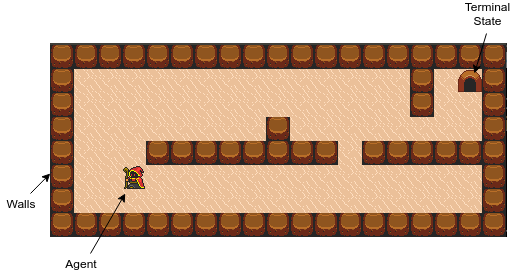
\includegraphics[width=0.5\textwidth]{./figures/env_sample}
\caption{The VGDL (Video Game Definition Language) environment example} 
\label{VGDL_sample}
\end{figure}

We use the Video Game Definition Language (VGDL), which is a high-level description language for 2D video games providing a platform for computational intelligence research (\cite{Schaul2013}).
The VGDL allows users to easily craft their own environments, which makes us possible to do various experiments without relying on a default environment. The VGDL platform provides an interface with OpenAI Gym (\cite{Brockman2016}), which is a commonly used benchmark platform.
The base game is a simple maze as shown in Figure \ref{VGDL_sample}.
There are 3 different types of cells: a goal cell, walls and paths. The agent can take 4 different actions: up, down, right and left.
The environment is not known to the agent in advance, and it attempts to find the goal by exploring the environment.
In all experiments, the agent receives -1 in any states except the goal state, where it gains a reward of 10.
Once the agent reaches the goal, or termination state, that episode is finished and the agent start the next episode from the starting point.

